%% git philosophy
%% Useful for bioinformatics services
%% Useful for software development
%% Differences with svn?


% ----------------------------------- slide


% The image shows how people think. 
% 1 - enthousiastic about Git
% 2 - developers familiar to SVN who are happy with it
% 3 - other developers who do not use VCS
\begin{frame}
\frametitle{Version Control System: from none to SVN to Git}
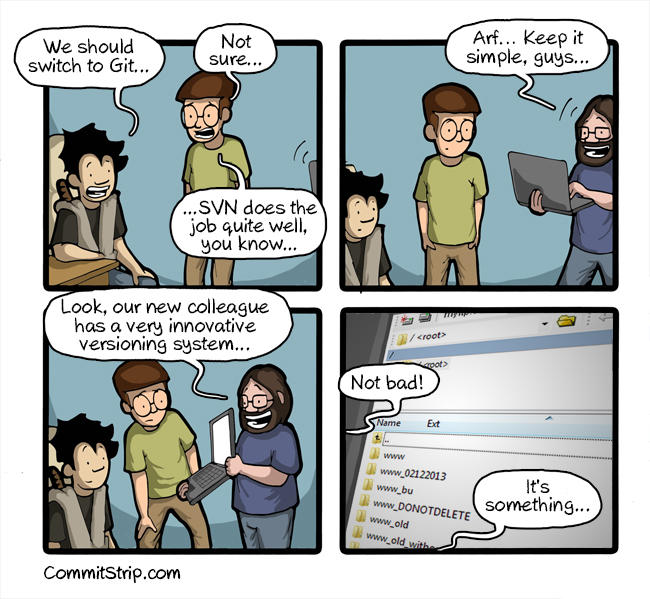
\includegraphics[height=0.9\textheight, width=\textwidth]{images/comics_intro}
\end{frame}


\begin{frame}
    \frametitle{Interest of Version Control System}
        \begin{block}{Sounds familiar ?}
    PI: \textit{Can you send me the script you used to generate this 
    figure last year ? The one where you fixed the important bug ? }\\
    \vspace{1em}
    you (maybe): \textit{Well, I only backup the version before the bug fix 
    and well you know ... but maybe it's in the dropbox in the directory 
    weekly\_backup\_march\_2015\_version2\_before\_noon ?}
        \end{block}
    
    \pause 

    \begin{alertblock}{Well it's time to move on and use a VCS}
        \begin{itemize}
        \item History
        \item Reproducibility
        \item Backup 
        \item Productive
        \item Not just for you but foundation for a team to collaborate
        \end{itemize}
    \end{alertblock}
\end{frame}

%on but be aware: \textbf{once you use version control
%tools, and any competent developers does, then they become a big part of your life !}


\begin{frame}
\frametitle{What is Version Control System anyway}
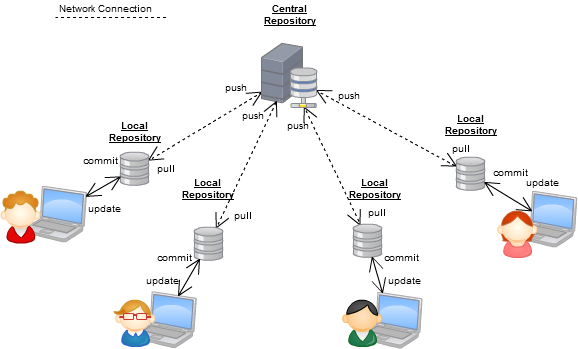
\includegraphics[height=0.9\textheight, width=\textwidth]{images/distributed}
\end{frame}


\begin{frame}
\frametitle{Which Version Control system shall I use ?}
\pause
\huge 
\begin{center}
GIT 
\end{center}
\end{frame}


\begin{frame}
\frametitle{Why Git 1/2 ?}
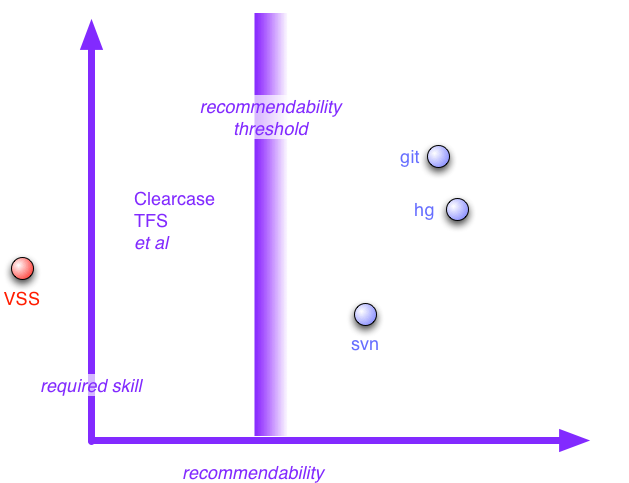
\includegraphics[height=0.9\textheight, width=\textwidth]{images/vcs-plane}
\end{frame}



\begin{frame}
\frametitle{Why Git 2/2 ?}

\begin{itemize}
\item Git is the most widely used VCS today. 
\item Most projects have moved from SVN to a Git
\item Every developer's working copy is also a repository with the full history
(distributed VCS).
\item Performance: faster than most of the concurrent \\
\item Security: hashing algorithm checks integrity of the code against accidental and malicious change\\
\item Flexible: support for various kinds of nonlinear development \textbf{branching}\\
\end{itemize}
\end{frame}


% ----------------------------------- slide
\begin{frame}
\frametitle{Motivation}

\begin{center}
The question is not why shall I use Git but How do we use it ?
\end{center}

\begin{center}
So let us start with some basics.
\end{center}

\end{frame}

